\documentclass[../../../main.tex]{subfiles}

\begin{document}
\subsection*{Appendix I: Laplace's Equation}

\subsubsection*{Separation Variable in Spherical Domain.} Next we will provide example of Laplace's equation in spherical coordinate, except I'm not gonna do that because it's too hard. We'll just skip to method of image.

\subsubsection*{Separation Variable in 2D Cartesian.} We will first discuss example for two-dimensional Laplace's Equation. Two infinite grounded metal plates lie parallel to the $x z$ plane, one at $y = 0$, the other at $y = a$. The left end, at $x = 0$, is closed off with an infinite strip insulated from the two plates, and maintained at a specific potential $V_0(y)$. Find the potential inside this “slot.”
\begin{figure*}[ht]
    \centering
    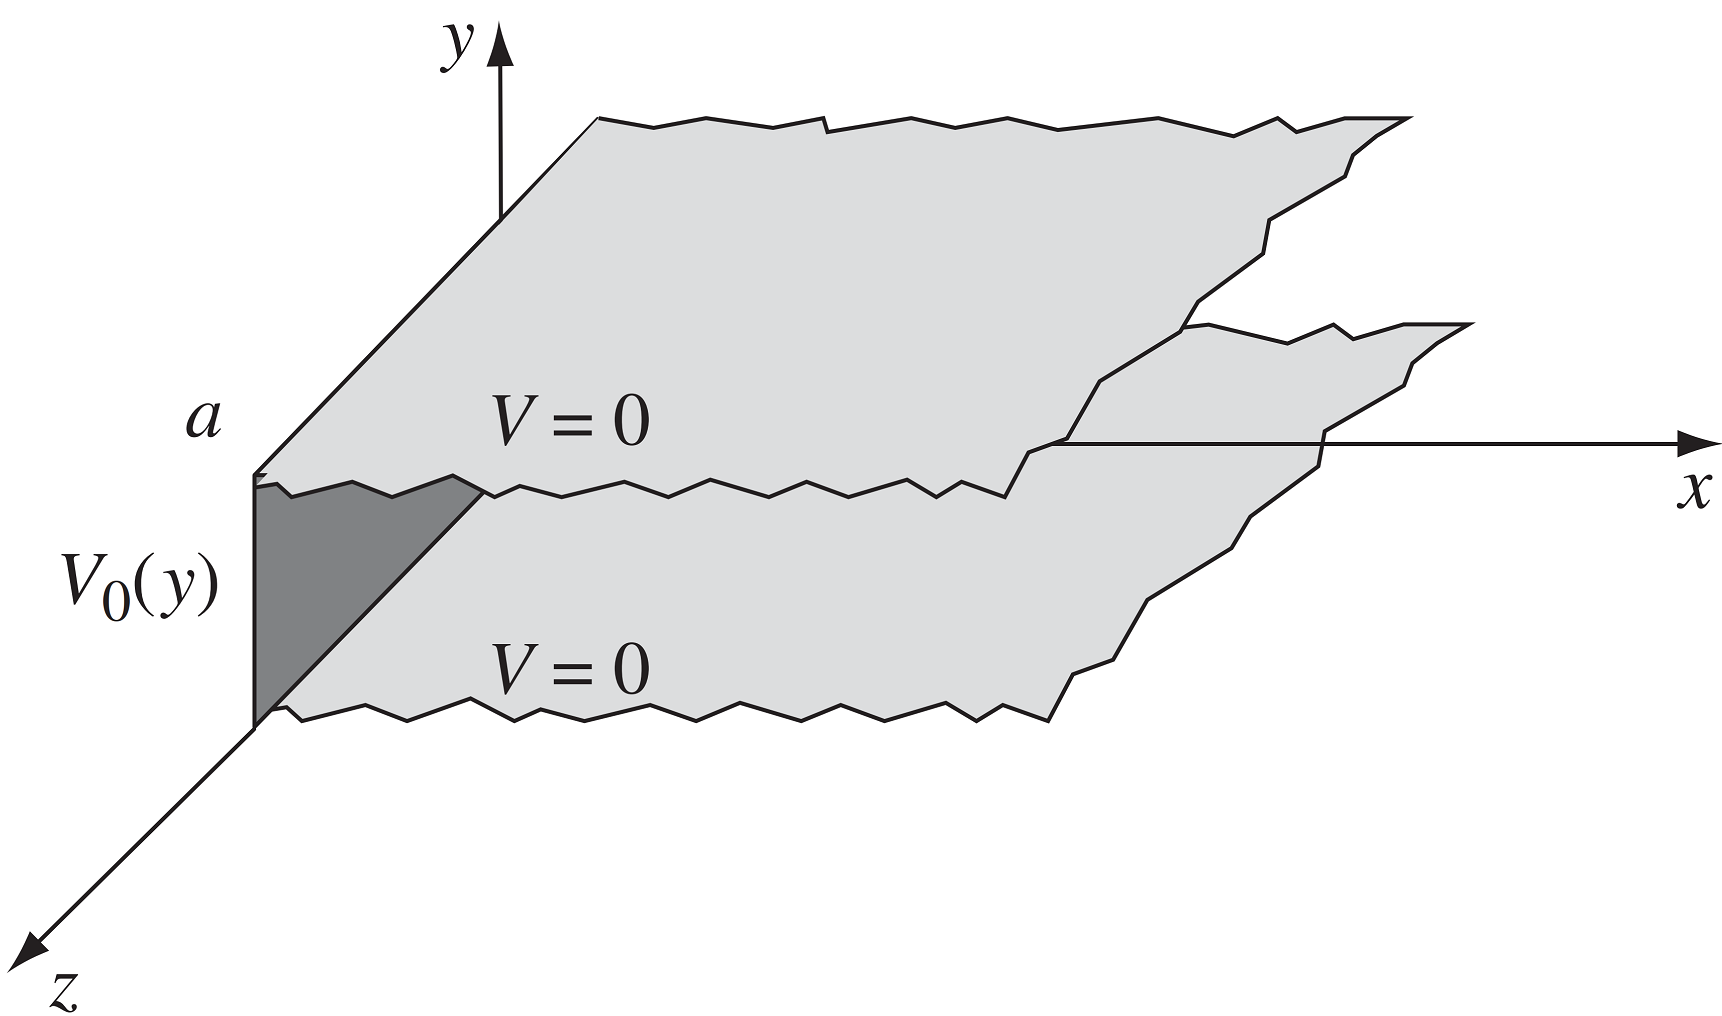
\includegraphics[height=4cm]{../Rss/Electromagnetism/Potential/CartesianSepVar.png}
\end{figure*}
The configuration is independent of z, so this is really a two-dimensional problem.
In mathematical terms, we must solve two-dimensional Laplace's equation subject to boundaries:
\begin{enumerate}
    \item $V = 0$ when $y = 0$,
    \item $V = 0$ when $y = a$,
    \item $V = V_0(y)$ when $x = 0$,
    \item $V \rightarrow 0$ as $x\rightarrow\inf $.
\end{enumerate}

Using the general solution, condition (4) requires that A equal zero. Absorbing B into C and D, we are left with
\begin{equation*}
    V(x,y)=e^{-kx}(C\sin ky+D\cos \cos ky)
\end{equation*}
Condition (1) now demands that D equal zero
\begin{equation*}
    V(x,y)=e^{-kx}C\sin ky
\end{equation*}
Meanwhile (2) yields $\sin ka = 0$, from which it follows that
\begin{equation*}
    k=\frac{n\pi}{a}\quad n=1,2,3,\ldots
\end{equation*}
The "generaler" solution is therefore
\begin{equation}\label{SolutEq}
    V(x,y)=\sum_{n=1}^{\infty}C_n\exp\bigg(-\frac{n\pi }{a}x\bigg)\sin \bigg(\frac{n\pi }{a}y\bigg)
\end{equation}
With the final boundaries condition (3)
\begin{equation*}
    V(0,y)=\sum_{n=1}^{\infty}C_n\sin \bigg(\frac{n\pi y}{a}\bigg)=V_0(y)
\end{equation*}
Using Fourier's Trick, i.e. multiply  by $\sin(n'\pi y/a)$ and integrate from 0 to a
\begin{equation*}
    \sum_{n=1}^{\infty}C_n\int_{0}^{a}\sin \bigg(\frac{n\pi y}{a}\bigg) \sin \bigg(\frac{n'\pi y}{a}\bigg)\;dy= \int_{0}^{a}V_0(y)\sin \bigg(\frac{n'\pi y}{a}\bigg)\;dy
\end{equation*}
Where the integrand on the left side is 0 if $n\neq n'$ and $a/2$ if $n= n'$. And the left side of equation reduces to $ (a/2)C n'$
\begin{equation}\label{SolutCoef}
    C_n=\frac{2}{a} \int_{0}^{a}V_0(y)\sin \bigg(\frac{n'\pi y}{a}\bigg)\;dy
\end{equation}
That does it: \ref*{SolutEq} is the solution, with coefficients given by \ref*{SolutCoef}. As a concrete example, suppose the strip at x = 0 is a metal plate with constant potential $V_0$. Then
\begin{equation*}
    C_n=\begin{cases}
        0,\quad \text{n is even}\\
        \dfrac{4V_0}{n\pi}, \quad \text{n is odd}
    \end{cases}
\end{equation*}
Thus
\begin{equation*}
    V(x,y)=\frac{4V_0}{\pi}\sum_{n=1,3,\dots}^{\infty}\frac{1}{n}\exp\bigg(-\frac{n\pi }{a}x\bigg)\sin \bigg(\frac{n\pi }{a}y\bigg)
\end{equation*}

\subsubsection*{Separation Variable in 3D Cartesian.} For the next question, we will discuss three-dimensional Laplace's Equation. For example, an infinitely long rectangular metal pipe (insides a and b) is grounded, but one end, at x = 0, is maintained at a specified potential $V_0(y, z)$. Find the potential inside the pipe. The boundaries conditions are therefore the following
\begin{enumerate}
    \item $V = 0$ when $y = 0$,
    \item $V = 0$ when $y = a$,
    \item $V = 0$ when $z = 0$,
    \item $V = 0$ when $z = b$,
    \item $V \rightarrow 0$ as $x \rightarrow \infty$,
    \item$ V = V_0(y, z)$ when $x = 0$
\end{enumerate}
\begin{figure*}[ht]
    \centering
    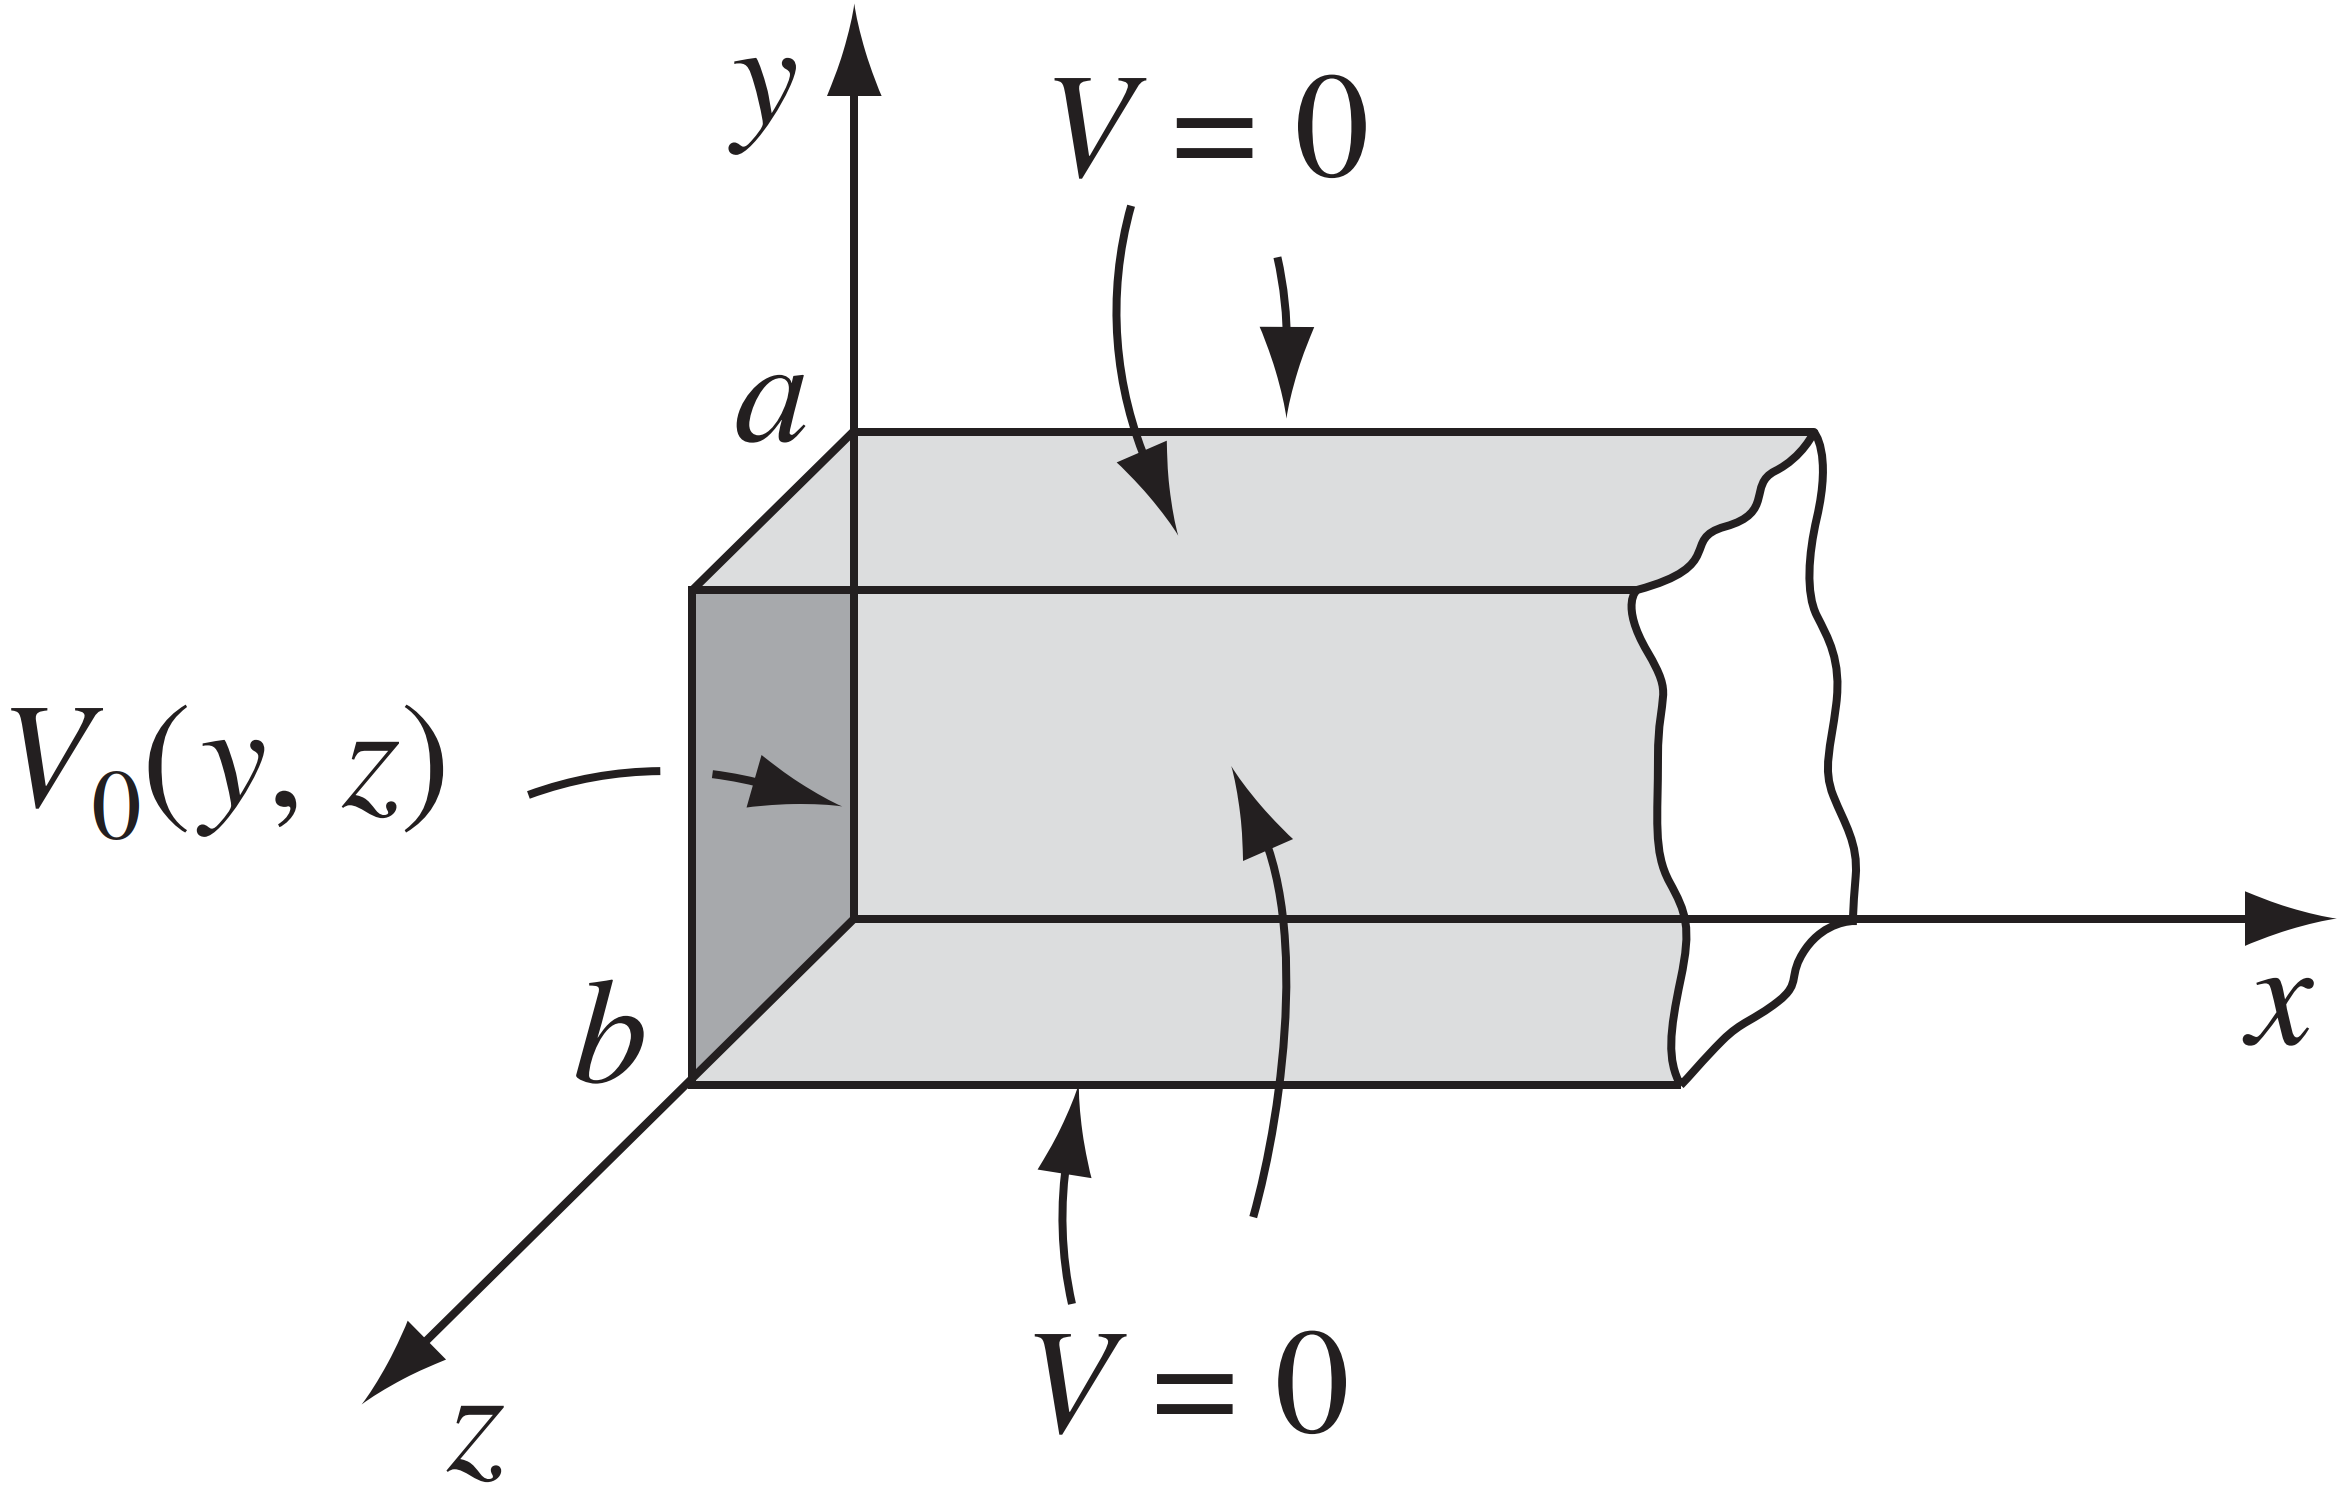
\includegraphics[height=4cm]{../Rss/Electromagnetism/Potential/CartesianSepVar2.png}
\end{figure*}

Boundary condition (5) implies $A = 0$, (1) gives $D = 0$, and (3) yields $F = 0$, whereas (2) and (3) require that $k = n\pi/a$ and $l = m\pi/b$, where $n$ and $m$ are positive integers. Combining the remaining constants, we are left with
\begin{equation*}
    V(x,y,z)=C\exp\biggl(-\pi\sqrt{(n/a)^2+(m/b)^2} x\biggr) \sin\biggl(\frac{n\pi y}{a}\biggr) \sin\biggl(\frac{m\pi z}{b}\biggr)
\end{equation*}
The generaler solution is then
\begin{equation}\label{SolutEq2}
    V=\sum_{n=1}^{\infty}\sum_{m=1}^{\infty}C_{n,m}\exp\biggl(-\pi\sqrt{\big(\frac{n}{a}\big)^2+\big(\frac{n}{b}\big)^2} x\biggr) \sin\biggl(\frac{n\pi y}{a}\biggr) \sin\biggl(\frac{m\pi z}{b}\biggr)
\end{equation}
We hope to fit the remaining boundary condition
\begin{equation*}
    V(0,y,z)=V_0(y,z)
\end{equation*}
or 
\begin{multline*}
    \sum_{n=1}^{\infty}\sum_{m=1}^{\infty}C_{n,m}\exp\biggl(-\pi\sqrt{\big(\frac{n}{a}\big)^2+\big(\frac{n}{b}\big)^2}x\biggr) \sin\biggl(\frac{n\pi y}{a}\biggr) \sin\biggl(\frac{m\pi z}{b}\biggr)\\=V_0(y,z)
\end{multline*}
To determine these constants, we multiply by $\sin(n'\pi y/a) \sin(m'\pi z/b)$ and integrate
\begin{multline*}
    \sum_{n=1}^{\infty}\sum_{m=1}^{\infty}C_{n,m} \int_{0}^{a}\sin\biggl(\frac{n\pi y}{a}\biggr) \sin\biggl(\frac{n'\pi y}{a}\biggr) dy \\\int_{0}^{b} \sin\biggl(\frac{m\pi z}{b}\biggr)\sin\biggl(\frac{m'\pi z}{b}\biggr)dz\\
    =\int_{0}^{a}\int_{0}^{b}V_0(y,z)\sin(n'\pi y/a) \sin(m'\pi z/b)\;dydz
\end{multline*}
Using Fourier's Trick, the left side is $(ab/4)C_{n,m} $, so
\begin{equation}\label{SolutCoef2}
    C_{n,m}=\frac{4}{ab}\int_{0}^{a}\int_{0}^{b}V_0(y,z)\sin(n'\pi y/a) \sin(m'\pi z/b)\;dydz
\end{equation}
Equation \ref{SolutEq2}, with the coefficients given by Eq. \ref{SolutCoef2}, is the solution to our problem.

\subsection*{Appendix II: Method of Image}
Suppose a point charge $q$ is held a distance $d$ above an infinite grounded conducting plane. Question: What is the potential in the region above the plane? 
\begin{figure*}[ht]
    \centering
    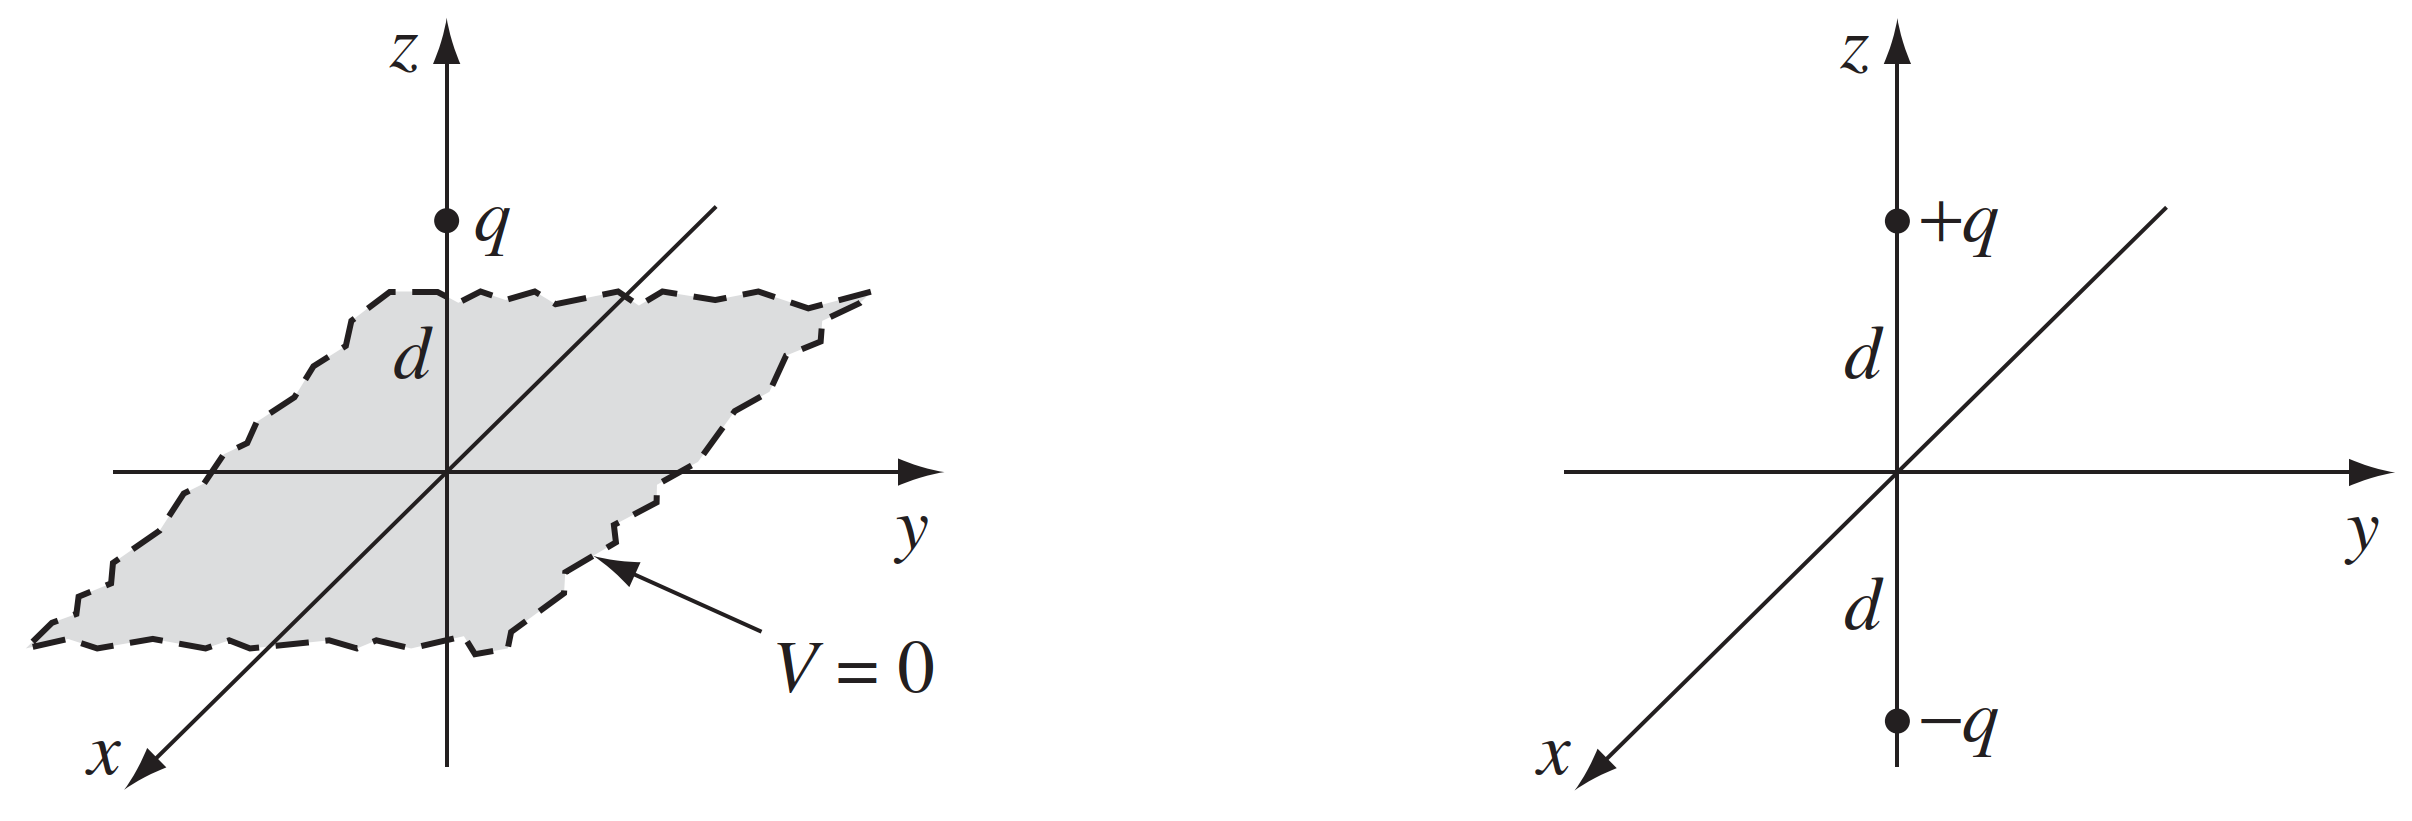
\includegraphics[width=\textwidth]{../Rss/Electromagnetism/Potential/MethIm.png}
    \caption*{Figure: Charge $q$ above grounded plane.}
\end{figure*}
Trick: Forget about the actual problem; we're going to study a completely different situation. This new configuration consists of two point charges, $+q$ at $(0, 0, d)$ and $-q$ at $(0, 0, -d)$, and no conducting plane. For this configuration, I can easily write down the potential:
\begin{equation*}
    V(x,y,z)=\frac{1}{4\pi\epsilon_0}\biggl(\frac{q}{\sqrt{x^2+y^2+(z-d)^2}}-\frac{q}{\sqrt{x^2+y^2+(z+d)^2}}\biggr)
\end{equation*}

It follows that:
\begin{enumerate}
    \item $V = 0$ when $ z = 0$, and
    \item $V \rightarrow 0$ for $x^2 + y^2 + z^2 \gg d^2$.
\end{enumerate}
Notice the crucial role played by the uniqueness theorem in this argument: If it satisfies Poisson's equation in the region of interest, and assumes the correct value at the boundaries, then it must be right.

Let us try another example. A point charge $q$ is situated a distance a from the center of a grounded conducting sphere of radius $R$. Find the potential outside the sphere.
\begin{figure*}[ht]
    \centering
    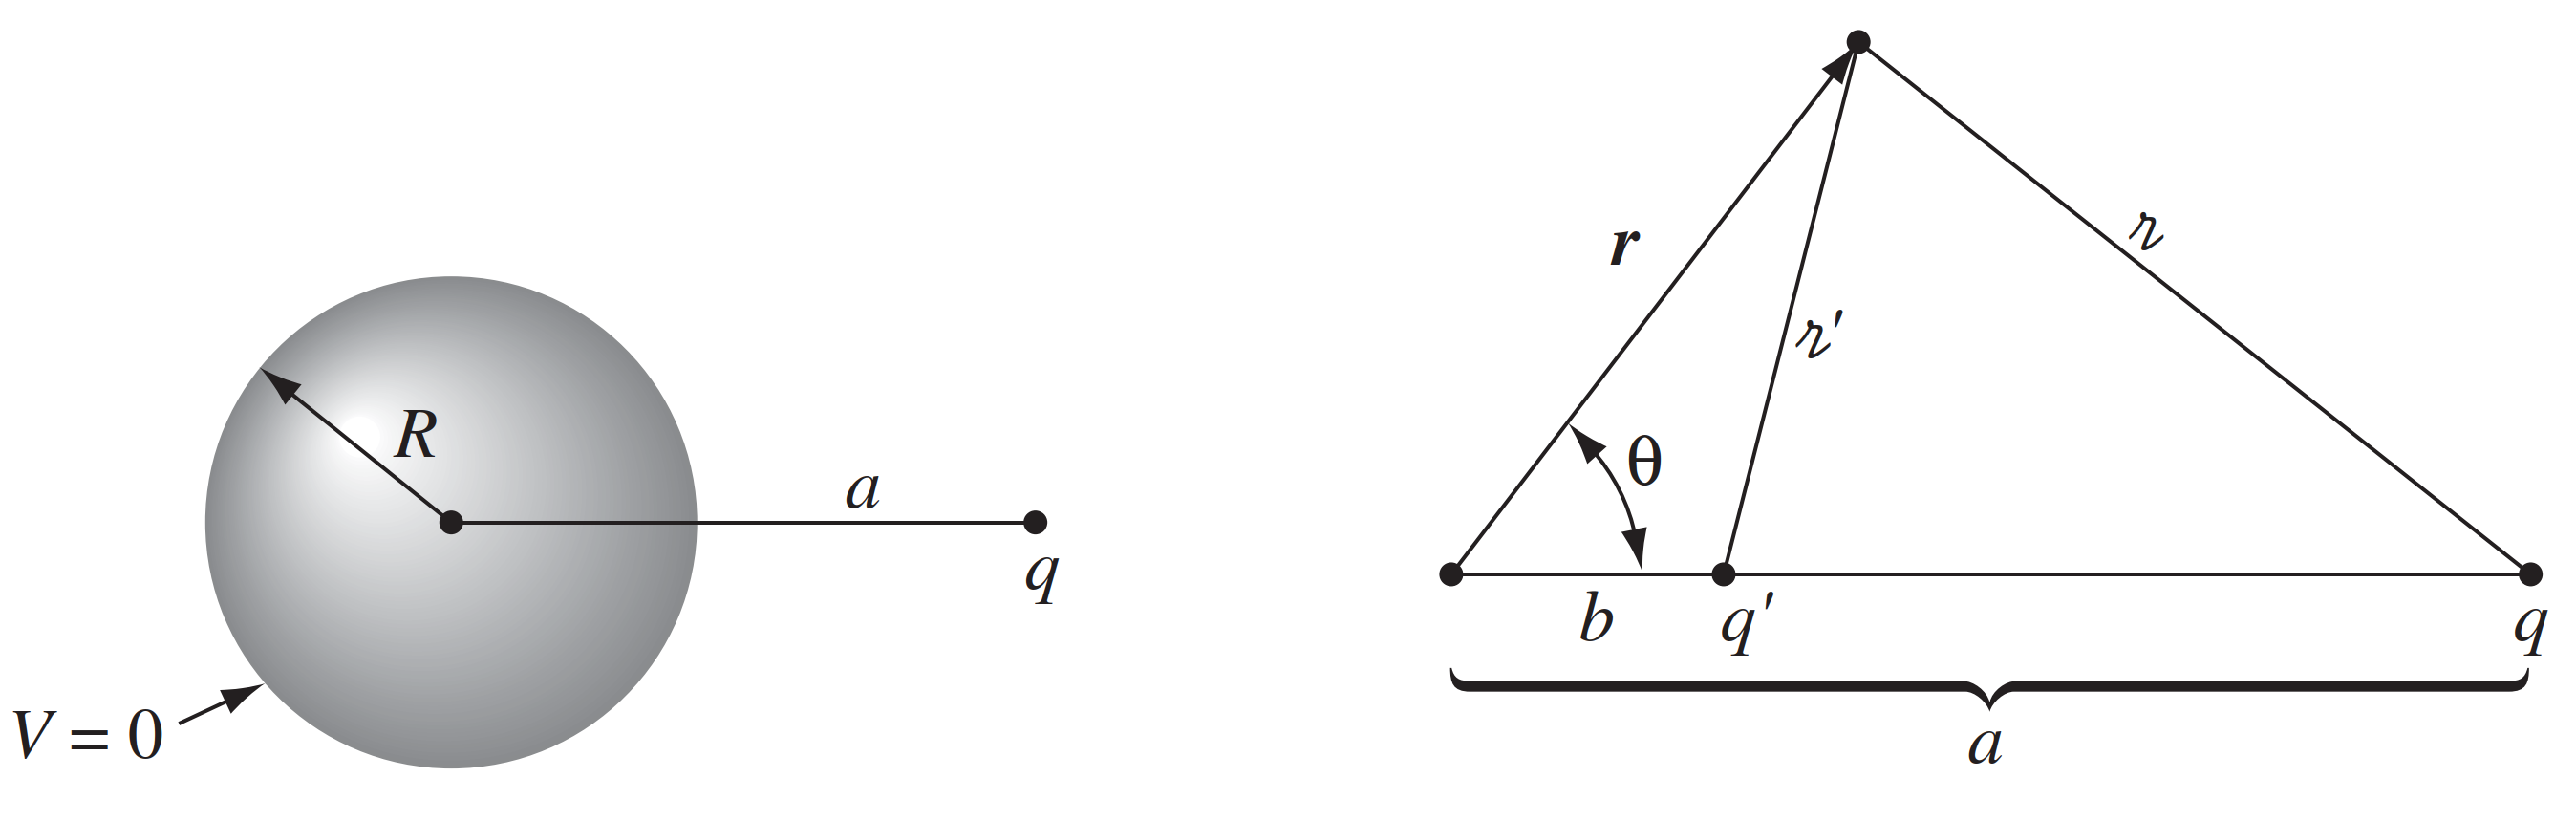
\includegraphics[width=\textwidth]{../Rss/Electromagnetism/Potential/MethIm2.png}
\end{figure*}
As before, we examine the completely different configuration, consisting of the point charge $q$ together with another point charge
\begin{equation*}
    q'=-\frac{R}{a}q
\end{equation*}
placed a distance
\begin{equation*}
    b=\frac{R^2}{a}
\end{equation*}
to the right of the center of the sphere. No conductor, now—just the two point charges. The potential of this configuration is
\begin{equation*}
    V(\mathbf{r})=\frac{1}{4\pi\epsilon_0}\biggl(\frac{q}{\rcurs}+\frac{q}{\rcurs '}\biggr)
\end{equation*}
where $r$ and $r'$ are the distances from $q$ and $q'$, respectively.
\end{document}